\documentclass[a4paper, 12pt]{article}

\usepackage[portuges]{babel}
\usepackage[utf8]{inputenc}
\usepackage[margin=1.0in]{geometry}
\usepackage{amsmath}
\usepackage{graphicx}
\usepackage{datetime}
\usepackage{enumerate}
\renewcommand{\baselinestretch}{1.5}

\emergencystretch 1pt%
\setlength{\parindent}{0pt}

\title{EFC2 - Classificação}
\author{Rafael Gonçalves - RA: 186062}
\date{}

\begin{document}


\maketitle

\section*{Parte I - Teoria Bayesiana de Decisão}

\begin{figure}[h!]
    \centering
    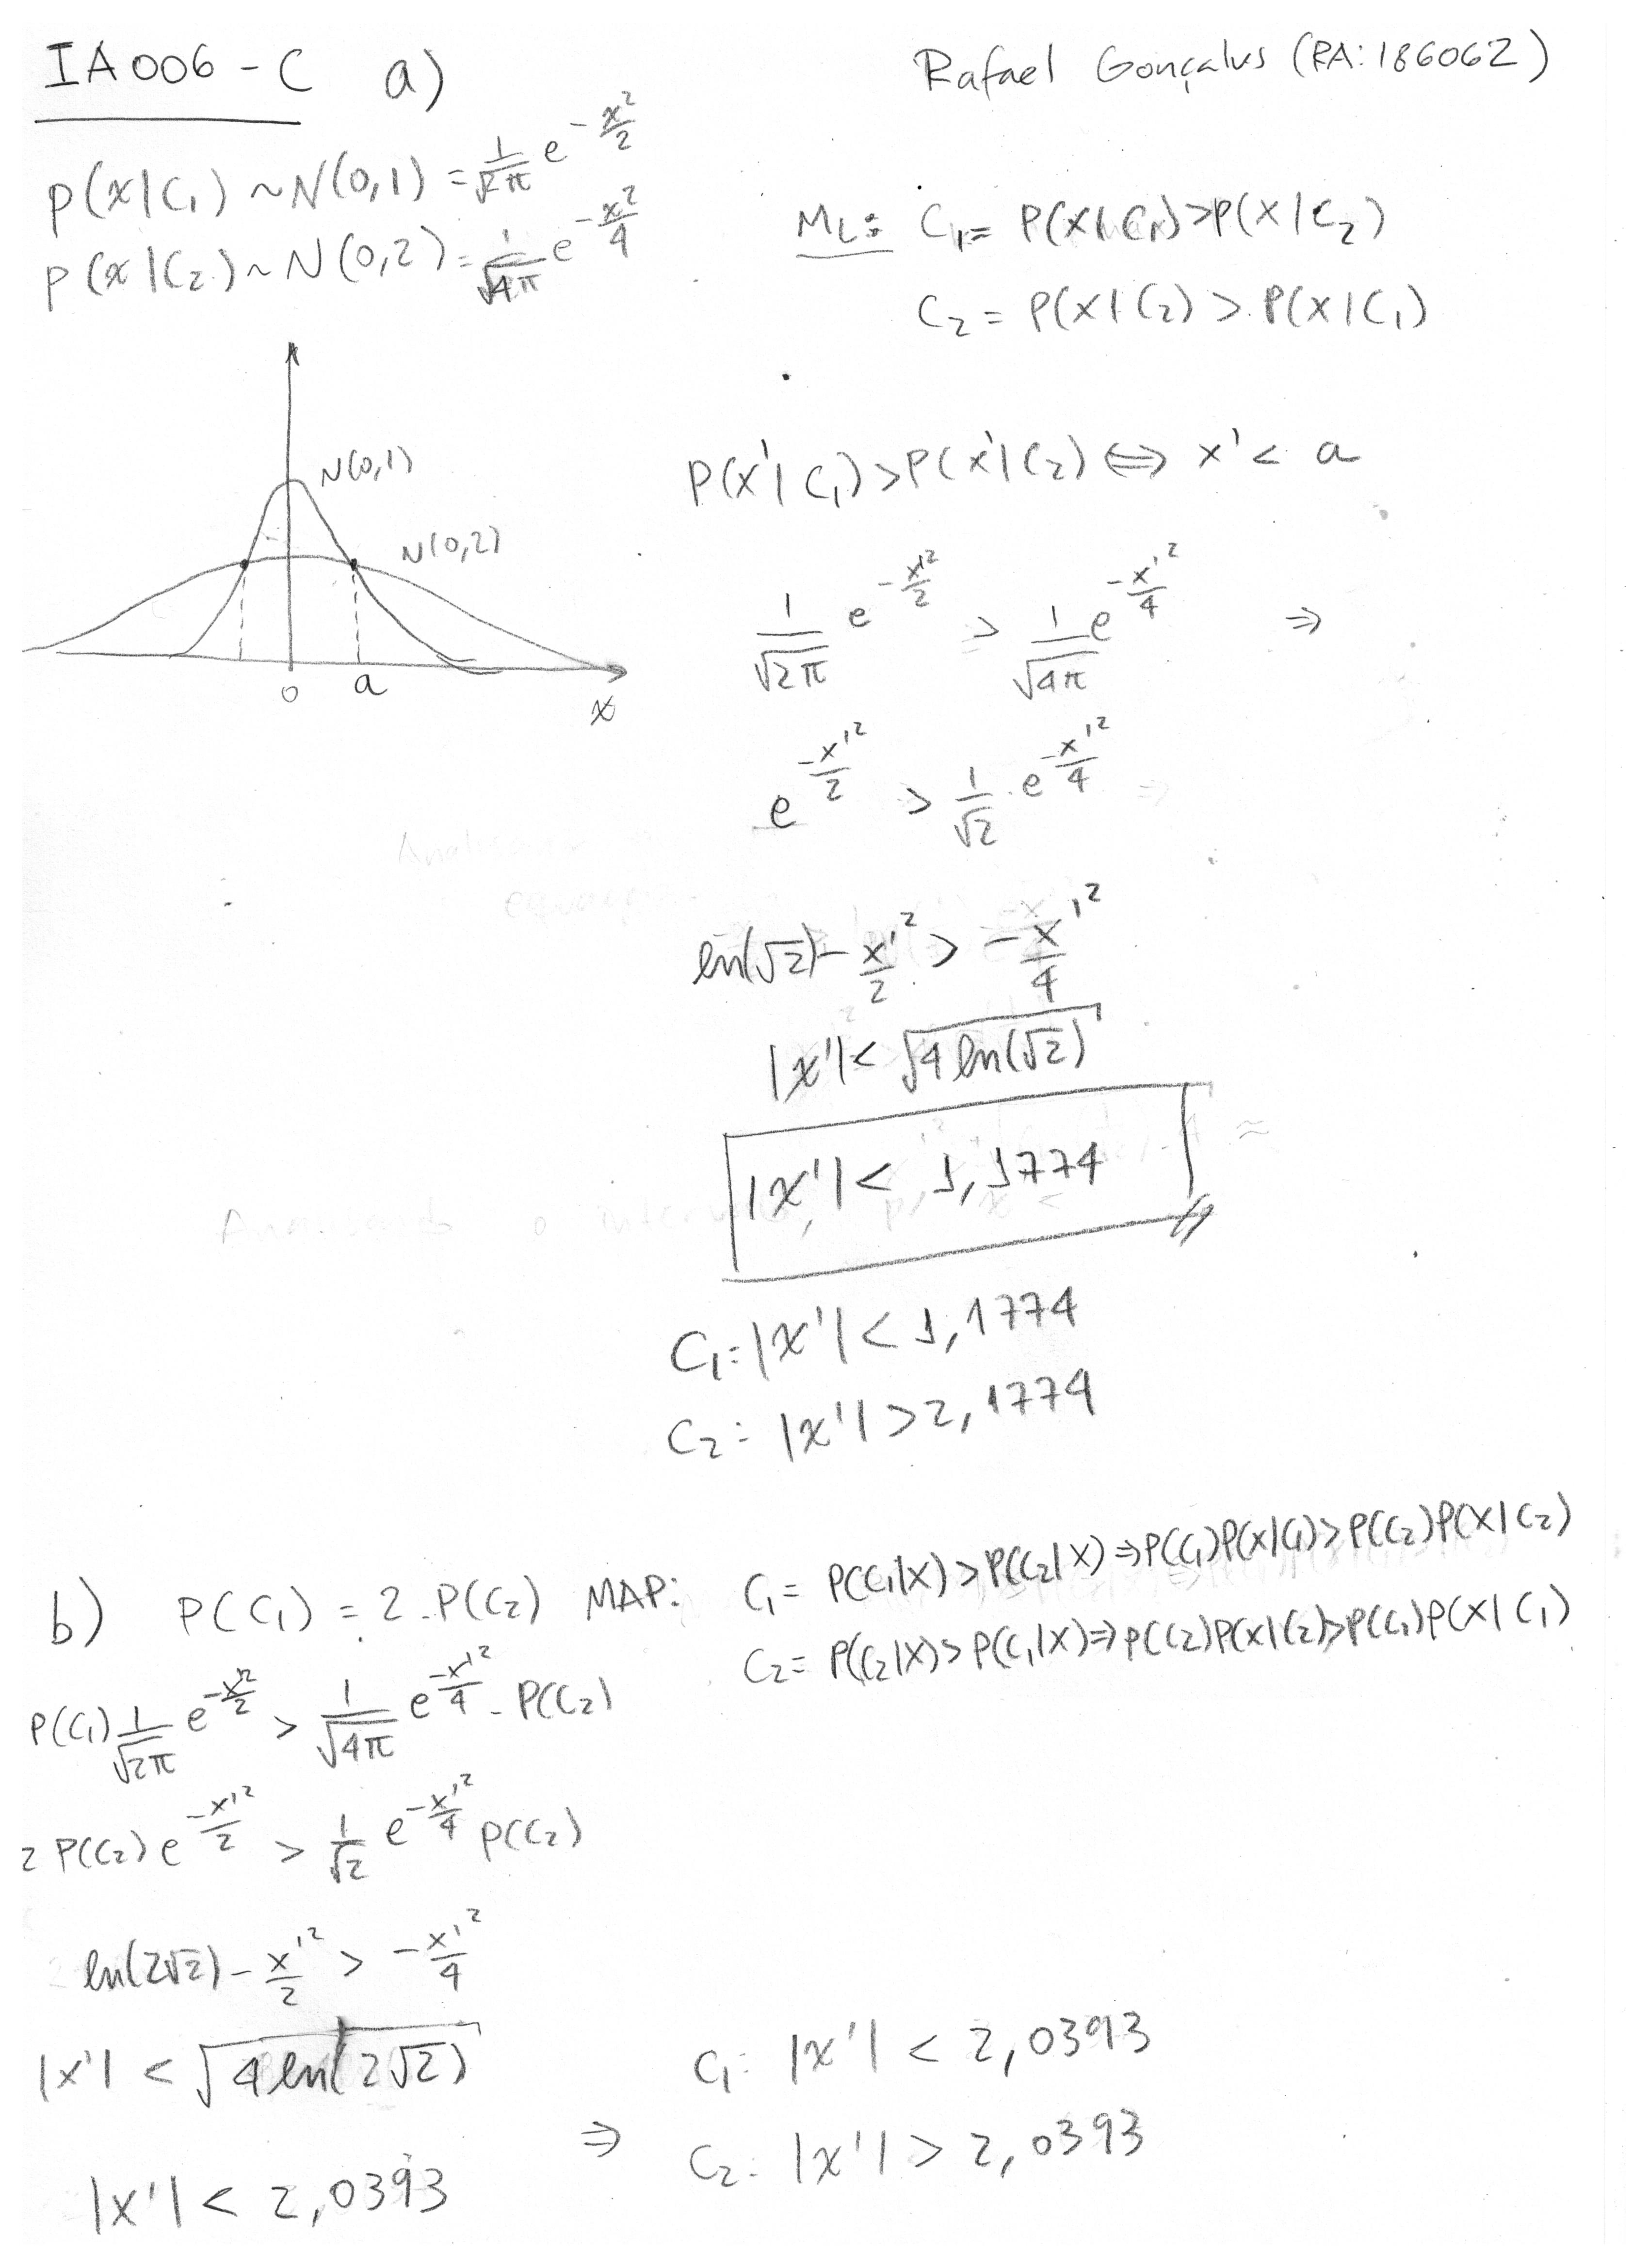
\includegraphics[width=1.0\textwidth]{images/parteI.png}
\end{figure}

\subsection*{c)}

Dado que o critério MAP leva em consideração a probabilidade a priori e o critério ML não, os resultados podem ser bem diferentes. Não é possível dizer com certeza neste caso, pois não sabemos em que intervalo se encontram os valores possíveis para 


\end{document}
